\documentclass[dvipsnames,authoryear,11pt]{article}


\usepackage{graphicx}
\usepackage{caption}
\usepackage{subcaption}

\usepackage{setspace}
%\doublespacing

%\usepackage{lineno}
%\linenumbers
%\modulolinenumbers[5]

\usepackage{amssymb}
\usepackage{booktabs}
\usepackage{algorithm,algorithmic}
\usepackage{amsmath}
\usepackage[english]{babel}
\usepackage[latin1]{inputenc}
%\usepackage[utf8]{inputenc}
\RequirePackage{natbib}
\usepackage{multirow}
\usepackage{arydshln}

\allowdisplaybreaks
\usepackage{geometry}
\geometry{a4paper,left=1in,right=1in,top=0.9in,bottom=1.3in}
\usepackage{tikz}
\usetikzlibrary{arrows,snakes,backgrounds}

\newtheorem{definition}{Definition}
\newtheorem{example}{Example}


\usepackage{amssymb}

\usepackage{amssymb}
\newcommand{\nb}[3]{
	{\colorbox{#2}{\bfseries\sffamily\scriptsize\textcolor{white}{#1}}}
	{\textcolor{#2}{\sf\small$\blacktriangleright$\textit{#3}$\blacktriangleleft$}}}
\newcommand{\version}{\emph{\scriptsize$-$Id$-$}}

% COMANDS TO LEAVE COMMENTS
\newcommand{\FL}[1]{\nb{FL}{blue}{#1}}

\newcommand{\refp}[1]{(\ref{#1})}




%opening


\title{The truck-and-freighter routing problem}
\author{ORO - Optimization in Trabnsportation and Logistics \\
	project at home }
\date{2017}

\begin{document}
	
	\maketitle

%	\begin{abstract}
		
%	\end{abstract}

\FL{Problelm introduction to be rewritten}

The truck-and-freighter routing problem consists in delivering goods starting from a principal distribution center to the multiple customers in a city. Within the city, there are 2 different areas. One is called vehicle-size regulated area and the other is called non-vehicle-size regulated area. To serve both areas, 2 different transports vehicles are available; a small truck (freighter) which will be able to reach both areas due to its size and lower CO2 emission, and a big truck which will serve only non-vehicle-size regulated area. In terms of capacity, a big truck will contain a significantly bigger capacity than the smaller truck. 
When a small truck has no loading goods, they will meet up the closest meeting point which will be located at a customer point which is located in the non-vehicle-size regulated area, furthermore; the small truck will be loaded again to continue delivering to the rest of the customers. The goal is strategically find the best routes, which includes also meeting points. At the end, all customers need to be reached by the optimal route minimizing the total distance covered and the transportation cost. 
	
	When both vehicles have completely covered all customers, they will need to meet again at a certain meeting point, finally; the big truck will carry the small one inside it, and come back to the main distribution center.
	

	
	\section{Problem description}
	
	In the truck-and-freighter routing problem (TFRP), we consider a distribution centre (DC) which takes index $0$.
	$J$ denotes the set of customers and $J^S \subset J$  is the subset of customers that can be served only by a feighter. 
	We denote by $P$ the set of parking nodes where coupling, decoupling and tranfers can occur between the freighter and the truck.
	The costs for both of vehicles are defined as $C_{ij}^B$, for a big truck, and $C_{ij}^S,$ for a small truck. $q_j$ represents the demand of each customer $j$. The capacities for each big and small trucks are defined as $Q_B$ and $Q_S$. 
	
		This problem is illustrated on Figure \ref{fig:fig1}.
		
	\begin{figure}[h]
		\centering
		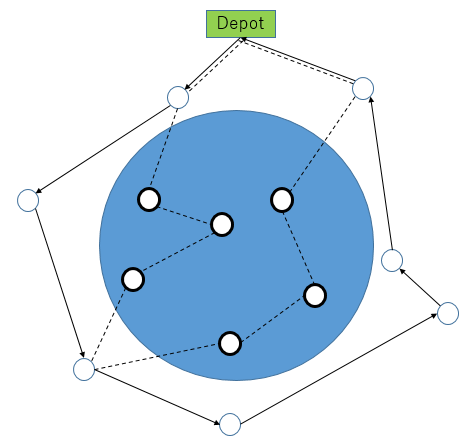
\includegraphics[width=0.6\linewidth]{figure}
		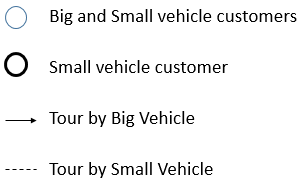
\includegraphics[width=0.3\linewidth]{legende}
		\caption{Problem Structure and Tour Types in the problem}
		\label{fig:fig1}
	\end{figure}
	
		
	
	\subsection{Assumptions}
	
	Following conditions are assumed,
	\begin{enumerate}
		\item	A small truck is considered as the only truck which can reach to customers in the vehicle-regulated area.
				The customers in non-vehicle-regulated area can be served by both big and small trucks.
		\item	To each of the trucks, one driver will be assigned.
		\item	Both big and small trucks must depart from depot and return to it at the same time. 
		\item	All different routes must be considered as a non-directed graph. Meaning that there is no restriction on the direction the truck might take.
		\item	All customer j must be visited at least once. 
		\item	Time window at each customer j is not considered.
	\end{enumerate}
	
	\section{Modeling the TFRP}
	
	\FL{The most important part below}
	
	\subsection{Sets and data}
	Sets: 
	\begin{itemize}
		\item $J=\{1,...,n\}$: set of customers.
		\item vertex $0$ and $n+1$ model the depot.
		\item $J_S \subset J$: nodes which can be served by the small truck only
		\item $J_B \subset J$: nodes which can be served by the large truck only
		\item $P$: set of transfer nodes 
		\item $V=\{0;n+1\} \cup J \cup P$
	\end{itemize}

	Data:
	\begin{itemize}
		\item $c_{ij}^B$: cost of going from node $i\in V$ to node $j \in V$ with the big truck
		\item $c_{ij}^S$: cost of going from node $i\in V$ to node $j \in V$ with the small truck alone
		\item $q_j$ demand of customer $j\in J$
		\item $Q^B, Q^S$ respective capacities of big and small trucks
		\item $t_{ij}$: time of traveling from node $i\in V$ to node $j \in V$
		\item $s_j$: duration of service at customer $j\in J$
		\item $[a_j,b_j]$: customer $j\in J$ time window
	\end{itemize}
	
\subsection{Model}	
	
Decision variables 
	\begin{itemize}
		\item ....
	\end{itemize}

	
	$$\textit{min }z=  \label{obj}$$
	such that:
	\begin{align}
		&\sum_{i \in J } X_{ijkl}& \forall j, k l \in ... \label{cte:cte1}\\
	\end{align}
	
\subsection{Comments}
 
The objective function states that ...

 
Constraints \refp{cte:cte1} state that ...


\section{Valid inequalities}

\section{Experimentations}




\end{document}
